% ============================================================================
% Chapter 3 · Methodology
% Style: no em dashes. Reasons before mechanics, plainly. One experiment, two
% instruments, one comparison against observation. Each concept introduced before use.
% ============================================================================

\section{Methodology}\label{sec:methodology}

\subsection{Rationale for a two-model approach}
\label{sec:design}

The rationale for building two models is a single comparison: one model is
constructed from first principles and the other learns from past trends, and
setting both against observed prices establishes which is better suited to
projecting a future that has not been observed. Furthermore, seeing if one is better suited for short term vs long term projection. More details on the logic flow of both models can be found in figure \ref{fig:architecture} and table \ref{tab:models}.

\begin{figure}[H]
    \centering
    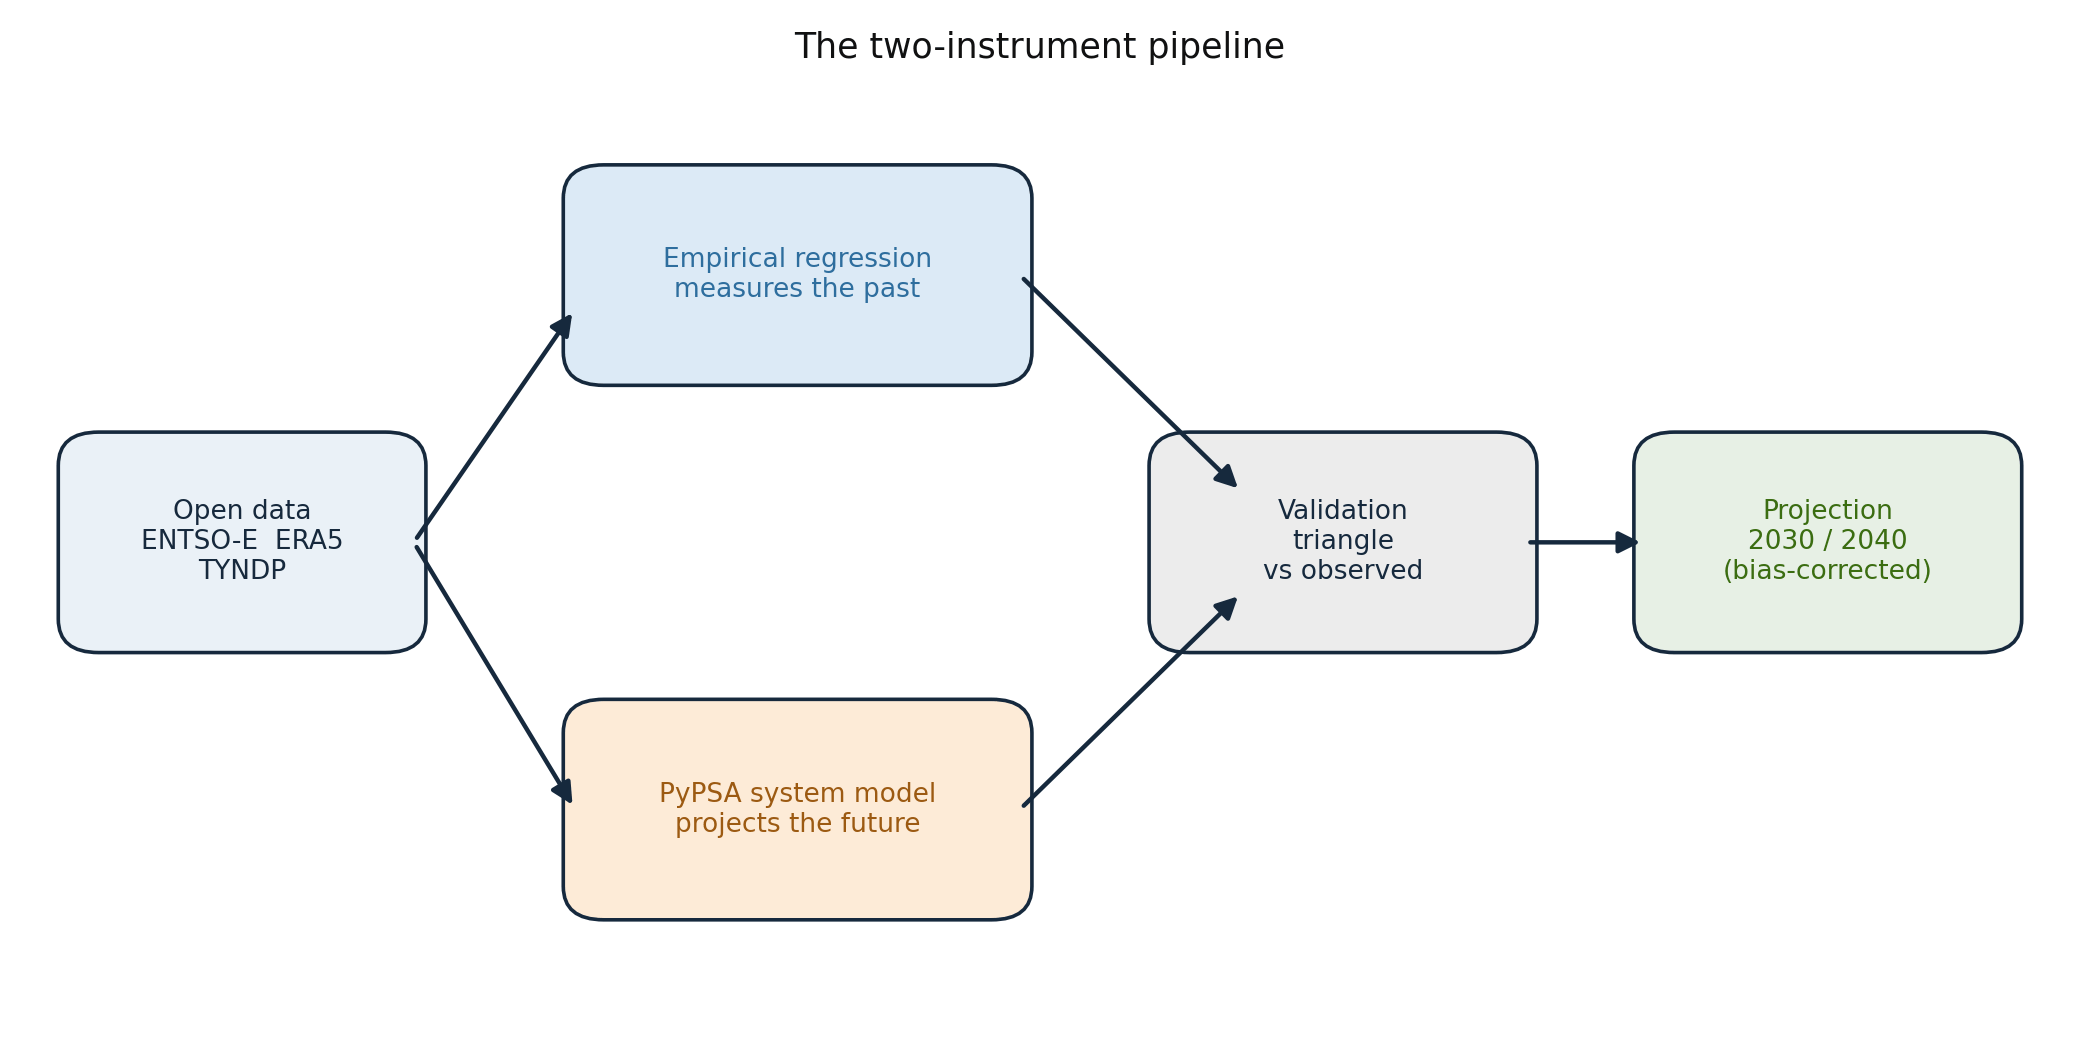
\includegraphics[width=0.95\textwidth]{architecture}
    \caption{The design of the thesis. Shared data feed the two models, both
    are compared against observed capture values, and the comparison decides
    which model is used for what.}
    \label{fig:architecture}
\end{figure}

\begin{table}[!htb]
\centering\small
\caption{How the two models are built, what they produce, and what each is used
for.}
\label{tab:models}
\begin{tabular}{p{2.7cm} p{5.6cm} p{5.6cm}}
\toprule
 & \textbf{Regression model} & \textbf{System model} \\
\midrule
Algorithm & Gradient-boosted trees (XGBoost) & Linear optimisation in PyPSA-Eur
(Gurobi) \\
\addlinespace
Built from & Seven market conditions, measured monthly for 31 farms from 2017 to
2024, giving 2{,}706 observations & The transmission grid, generation fleets,
ERA5 weather and TYNDP scenarios, solved hourly across thirty nodes \\
\addlinespace
Produces & Monthly capture value for each farm & Hourly prices and generation in
every zone, and annual capture value per zone \\
\addlinespace
Compared against & Observed capture value, with whole farms held out of the
fitting & Observed capture value in each zone and year \\
\addlinespace
Used for & Measuring the present and explaining the mechanism & Projecting 2030
and 2040, with its measured error subtracted \\
\bottomrule
\end{tabular}
\end{table}

\subsection{The use of capture value}
\label{sec:currency}

The regression
model applies it monthly to each farm, using day-ahead prices. The system model
applies it annually to each zone, using its own modelled prices. The comparison
of Section~\ref{sec:triangle} applies it to both against observation. In every
case it is calculated only over the hours for which both a price and a
generation figure exist, which is what makes the three sets of numbers
comparable. Denmark is treated as two zones throughout, DK1 and DK2.

One feature of the definition matters for what follows. Capture value depends on
the prices in a zone, weighted by when a farm generates. Prices are observed for
every zone in the study, and generation comes from the virtual wind farm of
Section~\ref{sec:vwf}, so a capture value can be measured for any zone with
observed prices, whether or not offshore wind operates there.

The regression model uses this to train on all seven enclosed Baltic zones
instead of the one zone with operating offshore wind. It weights prices that
have already occurred by a wind profile that has been validated against metered
output, so the only unobserved element is the farm itself. The projection in
Chapter 4 asks more than this, since it prices farms in markets that do not yet
exist.

\subsection{Data sources}\label{sec:data}

\subsubsection{Market data}\label{sec:market_data}

All market data come from the ENTSO-E Transparency Platform and cover 2017 to
2024. They comprise day-ahead prices for 22 bidding zones, hourly load, hourly
generation by technology, flows across 28 borders, and the yearly capacity of
each border. Everything is hourly and in UTC, and prices are resolved by bidding
zone rather than by country, so DK1, DK2 and SE4 are separate.

The platform under-reports Dutch renewable generation, which is therefore
rescaled to match physical capacity factors while keeping its hourly shape
\cite{Jacquet2024}, and British day-ahead prices cease publication after
Brexit, so the three British farms contribute only up to 2020. No other
corrections are applied to the market data.

\subsubsection{Meteorological and wind farm data}\label{sec:farm_data}

The study covers 31 offshore wind farms, sixteen in the North Sea and fifteen in
the Baltic, including sites that are operating, under construction and planned.
The operating farms are the ones whose modelled generation can be checked
against metered output, and they are used for validation. Every site in a zone
with observed prices is used to fit the regression model, whether it is
operating or not (Section~\ref{sec:fitting}).

A farm belongs to the sea its foundations stand in. DK2 and SE4 are part of the
Nordic synchronous area, but their farms stand in the western Baltic, experience
Baltic weather, and sell into the same enclosed market as the Polish and
Baltic-state fleets, so they are treated in this work as Baltic.

Within that geography the analysis uses four groups, kept the same throughout.
The open \textbf{North Sea} is the reference: Germany, the Netherlands, Belgium,
DK1 and France. The \textbf{under-built} Baltic is Poland, Estonia, Latvia and
Lithuania, which have very little offshore wind built so far. The
\textbf{built-out} Baltic is DK2 and SE4, which already have offshore wind in
operation. \textbf{Finland} is kept separate, because its low capture value
comes from nuclear generation holding prices down rather than from wind. The
groups are chosen so that the built-out zones show today what the under-built
ones are heading towards.

Hourly wind speeds at 10 and 100 metres come from ERA5, the fifth-generation
reanalysis of the European Centre for Medium-Range Weather Forecasts, taken at
each farm's nearest 0.25 degree grid cell. A reanalysis is a modern weather
model re-run over the past and combined with every available observation, and it
is the standard source of wind data for energy studies. ERA5 is known to
underestimate the strongest offshore winds \cite{Gandoin2024}. These speeds are left uncorrected, because the power-curve adjustment of
Section~\ref{sec:vwf} corrects the average level only, and the validation
reported there tests whether the resulting output is nonetheless accurate.

\subsubsection{Scenario data}\label{sec:scenario_data}

Future capacities, demand, fuel and carbon prices and battery fleets come from
the 2024 Ten-Year Network Development Plan, the official scenario framework of
the European transmission system operators \cite{TYNDP2024}. They are extracted
once into a single set of per-country tables, which both models then use. Because these tables cover renewable technologies only, the thermal capacity
they omit, and the corrections that omission requires, are set out in
Section~\ref{sec:projection}.

\subsection{The regression model}\label{sec:empirical}

\subsubsection{Virtual wind farm model}\label{sec:vwf}

Most of the farms in the study are not yet built, so generation is modelled for
every site, including those already operating. The method follows Staffell and
Pfenninger \cite{Staffell2016} as adapted by Jacquet \cite{Jacquet2024}, in
three steps.

\begin{enumerate}
    \item \textbf{Height extrapolation.} ERA5 gives wind speed at 10 and 100
    metres, and the IEA 15~MW reference turbine used has a hub height of
    150 metres \cite{Gaertner2020}. Speed is carried up to that height by
    fitting a logarithmic profile through the two known levels,
    %
    \begin{equation}
        u(z) = u_{\mathrm{ref}}\,\frac{\ln(z/z_0)}{\ln(z_{\mathrm{ref}}/z_0)},
        \label{eq:log_wind}
    \end{equation}
    %
    where $u(z)$ is the speed at height $z$, $z_{\mathrm{ref}}$ is a height at
    which the speed is known, and the surface roughness $z_0$ is solved from the
    10 and 100 metre pair. This is the standard description of how friction at
    the sea surface slows the wind near it and lets speed increase with height.

    \item \textbf{Power conversion.} Speed is turned into power using the
    turbine's power curve, which rises steeply between the cut-in speed of
    3~m\,s$^{-1}$ and the rated speed near 10.6~m\,s$^{-1}$, then stays flat up
    to the cut-out speed of 25~m\,s$^{-1}$. Output is set to zero outside that
    range, so neither calm nor storm hours produce anything.

    \item \textbf{Fleet adjustments.} Two corrections are applied, both
    calibrated by Hayes et al.\ on metered European farms \cite{Hayes2021}. The
    curve is smoothed ($\sigma = 1.17$~m\,s$^{-1}$), because the turbines across
    a single farm do not all meet the same wind speed, and it is shifted towards
    higher speeds ($w_0 = 0.71$~m\,s$^{-1}$) to account for wake losses and for
    the ERA5 bias noted above (Figure~\ref{fig:power_curve}).
\end{enumerate}

\begin{figure}[!htb]
    \centering
    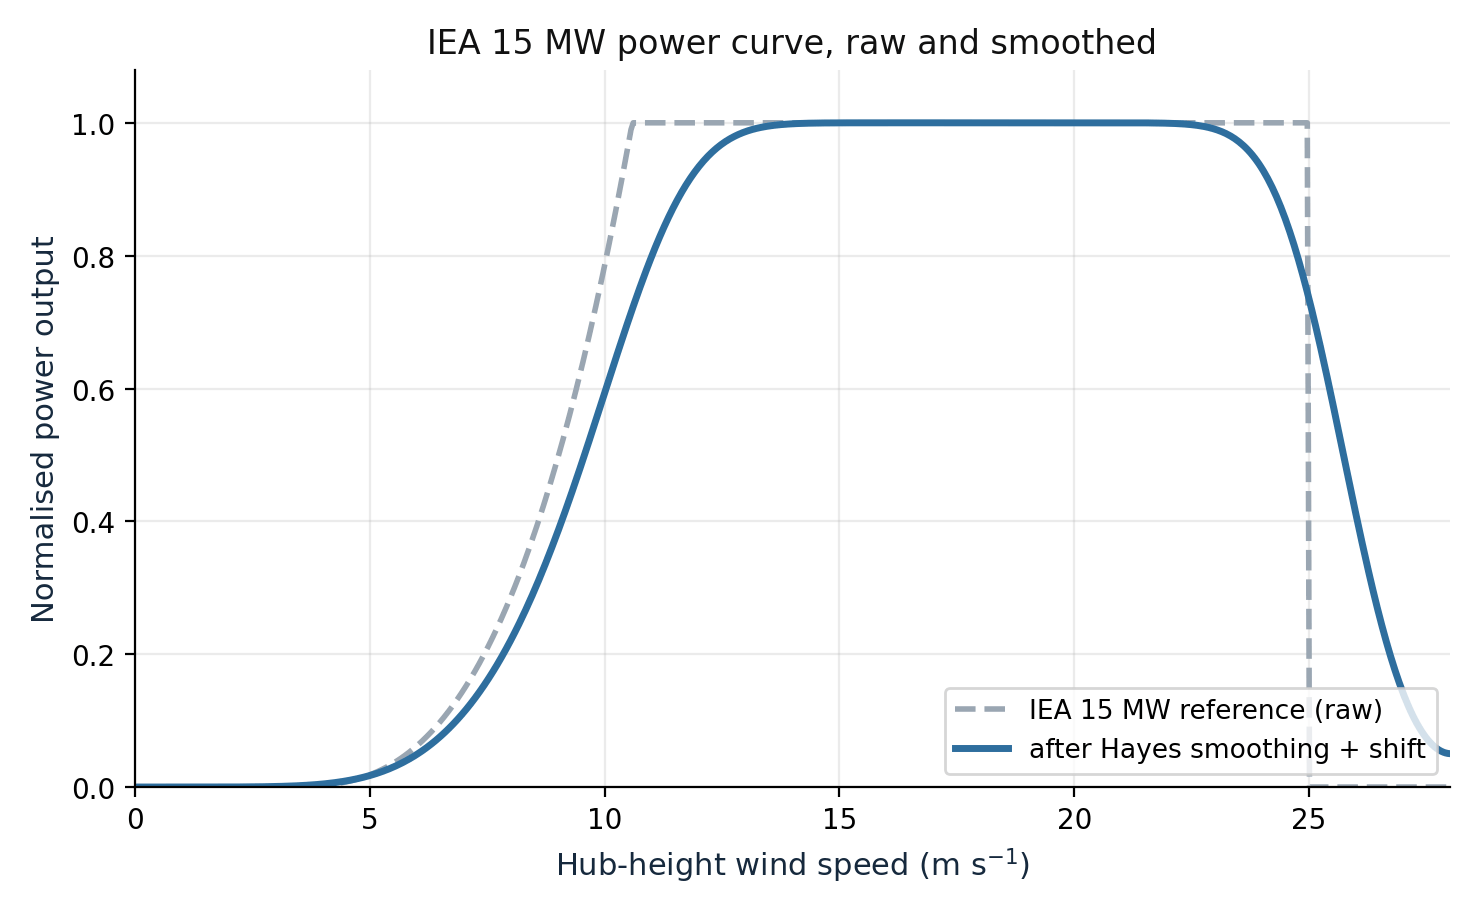
\includegraphics[width=0.62\textwidth]{power_curve}
    \caption{The IEA 15~MW reference power curve before and after the two
    adjustments, used to convert wind speed at hub height into output. Smoothing
    $\sigma=1.17$~m\,s$^{-1}$, shift $w_0=0.71$~m\,s$^{-1}$.}
    \label{fig:power_curve}
\end{figure}

The modelled generation is then checked against metered output. Aggregated to
zone level, the modelled farms reach a median hourly correlation of 0.88 with
the generation ENTSO-E reports, and 0.95 monthly, across five zones and three
years (Figure~\ref{fig:vwf_vs_observed}).

\begin{figure}[!htb]
    \centering
    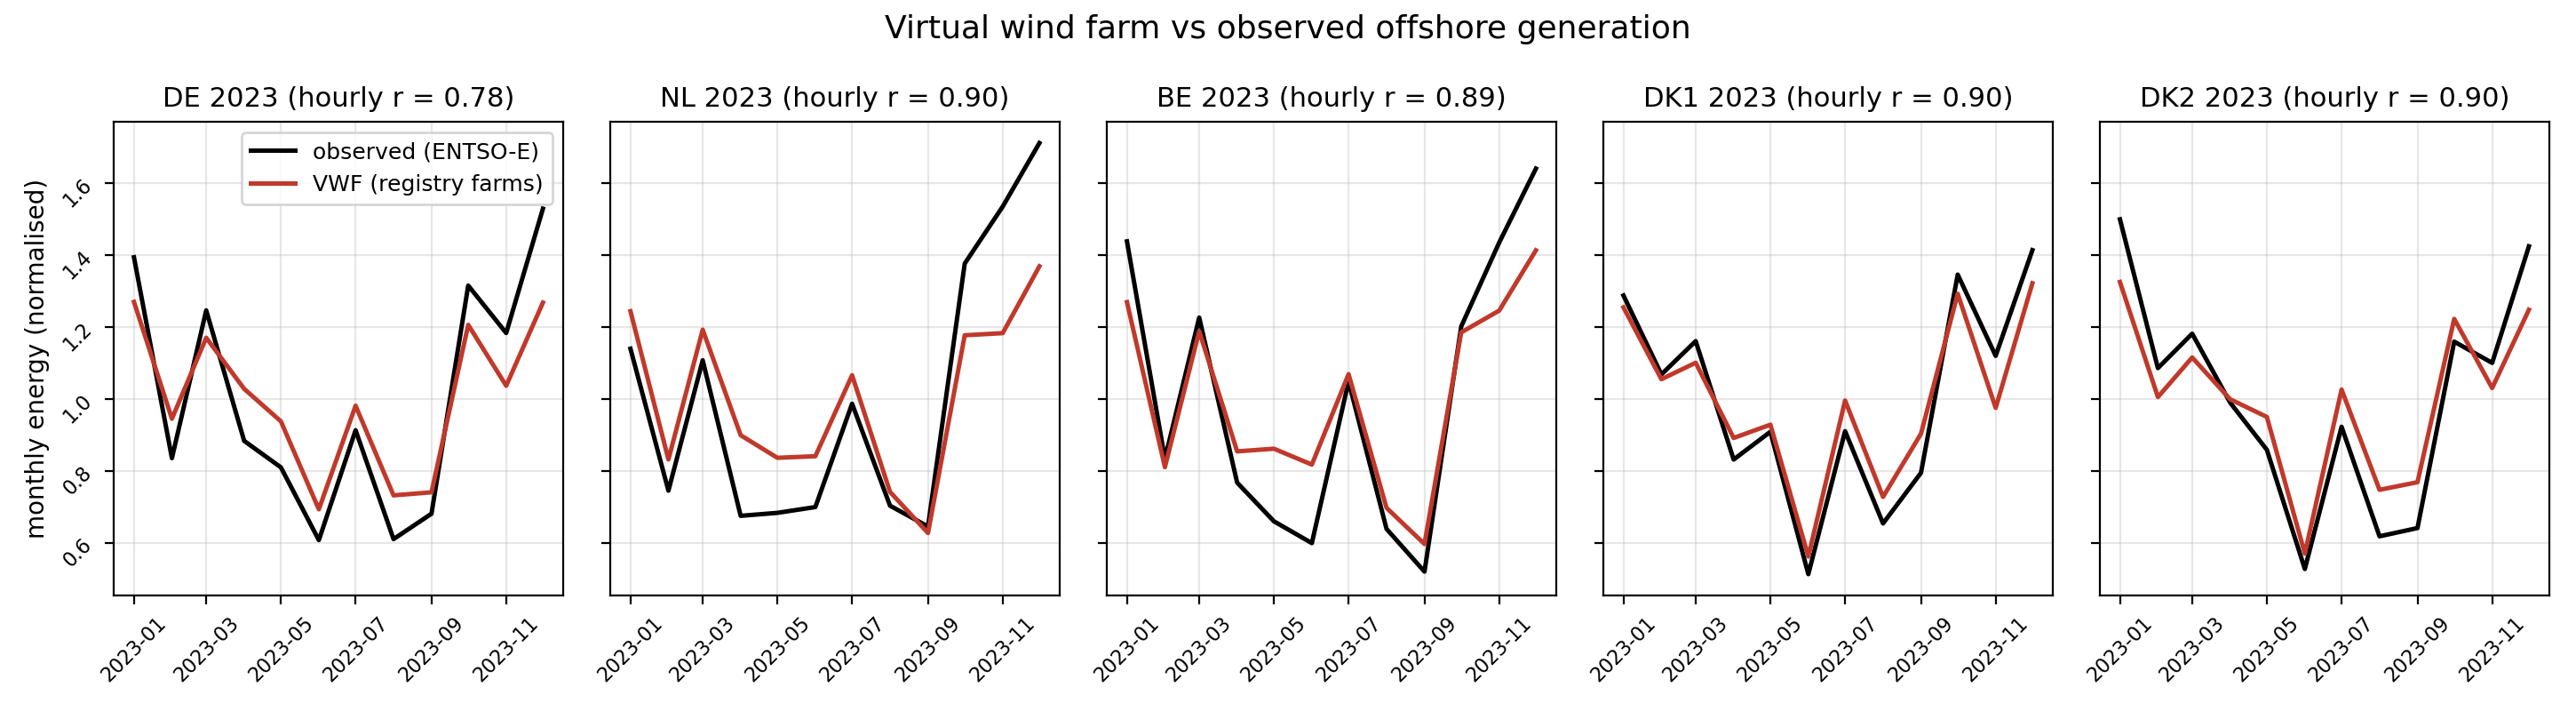
\includegraphics[width=0.95\textwidth]{fig_vwf_vs_observed}
    \caption{The modelled wind farms checked against observed offshore
    generation in 2023. Monthly energy from the modelled farms, normalised
    (red), against the metered fleet in the same zone (black). The median hourly
    correlation is 0.88 and the monthly correlation 0.95.}
    \label{fig:vwf_vs_observed}
\end{figure}

The timing of the output is what matters, because capture value weights
prices by when a farm generates. The modelled output does sit above the metered
figures in absolute terms, since it does not subtract every loss a real farm
incurs. This difference in level does not affect the results, because capture value is
a ratio with generation on both sides, and the farm enters the model's inputs
only through correlations, which are unchanged when output is scaled; a
constant error in the level therefore cancels.


\subsubsection{Feature set at bidding zone resolution}\label{sec:features}

Each farm-month gets seven features, following Jacquet's design
\cite{Jacquet2024} with one upgrade, resolution: each is computed for the farm's
\textit{market area}, the bidding zone where zone-resolved data exist (DK1, DK2,
SE4) and the country elsewhere, so the seven Danish farms see DK1 and DK2
conditions rather than a Danish average. Together they turn the cannibalisation
mechanism of Section~\ref{sec:value_problem} into measurable quantities: how
crowded the farm's selling hours are, how exposed its market is, and how much
surplus the system can absorb.

Features 1 and 2 are the hourly correlations of the farm's output with its
area's total variable renewable generation and with its load,
%
\begin{equation}
    \rho^{\mathrm{VRE}}_{f,m} = \mathrm{corr}\bigl(g_{f,t},\,
    G^{\mathrm{VRE}}_{z,t}\bigr), \qquad
    \rho^{\mathrm{load}}_{f,m} = \mathrm{corr}\bigl(g_{f,t},\,
    L_{z,t}\bigr), \qquad t \in m.
    \label{eq:correlations}
\end{equation}
%
The first measures crowding, a farm producing when every other renewable
produces selling into depressed prices; the second measures alignment with
demand, which lifts value. They enter separately so Chapter 4 can read their
contributions apart; their signed difference forms the pattern penalty in the
analytical equation of Section~\ref{sec:mechanism_tools}. Feature 3 is
penetration, the monthly renewable market share $S_{z,m} =
E^{\mathrm{VRE}}_{z,m} / E^{\mathrm{load}}_{z,m}$, which locates the market on
the cannibalisation curve. Features 4 and 5 are monthly gas and carbon prices,
which set the level of the thermal merit order and so how far prices fall when
wind displaces it. Feature 6 is flexibility, storage capacity over renewable
capacity, the system's ability to move surplus out of windy hours.

Feature 7 is interconnection, and it departs from both predecessors on
Efthymiadou's evidence that realised interconnector \emph{utilisation} rather
than installed capacity dampens price volatility
\cite{Efthymiadou2025, Jacquet2024}:
%
\begin{equation}
    I_{\mathrm{int},z} =
    \frac{\sum_{b}\, \overline{|F_{b}|}}{\sum_{b}\, \max_{t} |F_{b,t}|},
    \label{eq:interconnection}
\end{equation}
%
the mean absolute flow on each external border, divided by that border's
capacity and summed across borders. The economic logic is that an
interconnector relieves cannibalisation only when it carries the
windy-hour surplus out of the zone, so its use and not its rated size is what
lifts capture value. Exact definitions, the dropped neighbour-synchronicity
discount and the index's limitations are recorded in
Appendix~\ref{app:assumptions}.

The two models represent cannibalisation differently: the regression model
encodes it through these features, learned from data, while in the system model
it emerges by construction as added wind shifts the merit order. Collinearity is
clean (largest variance inflation factor 2.16), so the feature contributions in
Chapter 4 read as near-independent mechanisms.
% VIF recomputed on the current 2,706-row panel: max 2.16 (carbon), feature 7 = 1.21.
Figure~\ref{fig:fig_C_feature_evolution} shows how each of the seven has moved
since 2017, averaged within each basin. This is the record the model learns
from, and the starting point from which the projection of
Section~\ref{sec:reg_projection} moves them.

\begin{figure}[!htb]
    \centering
    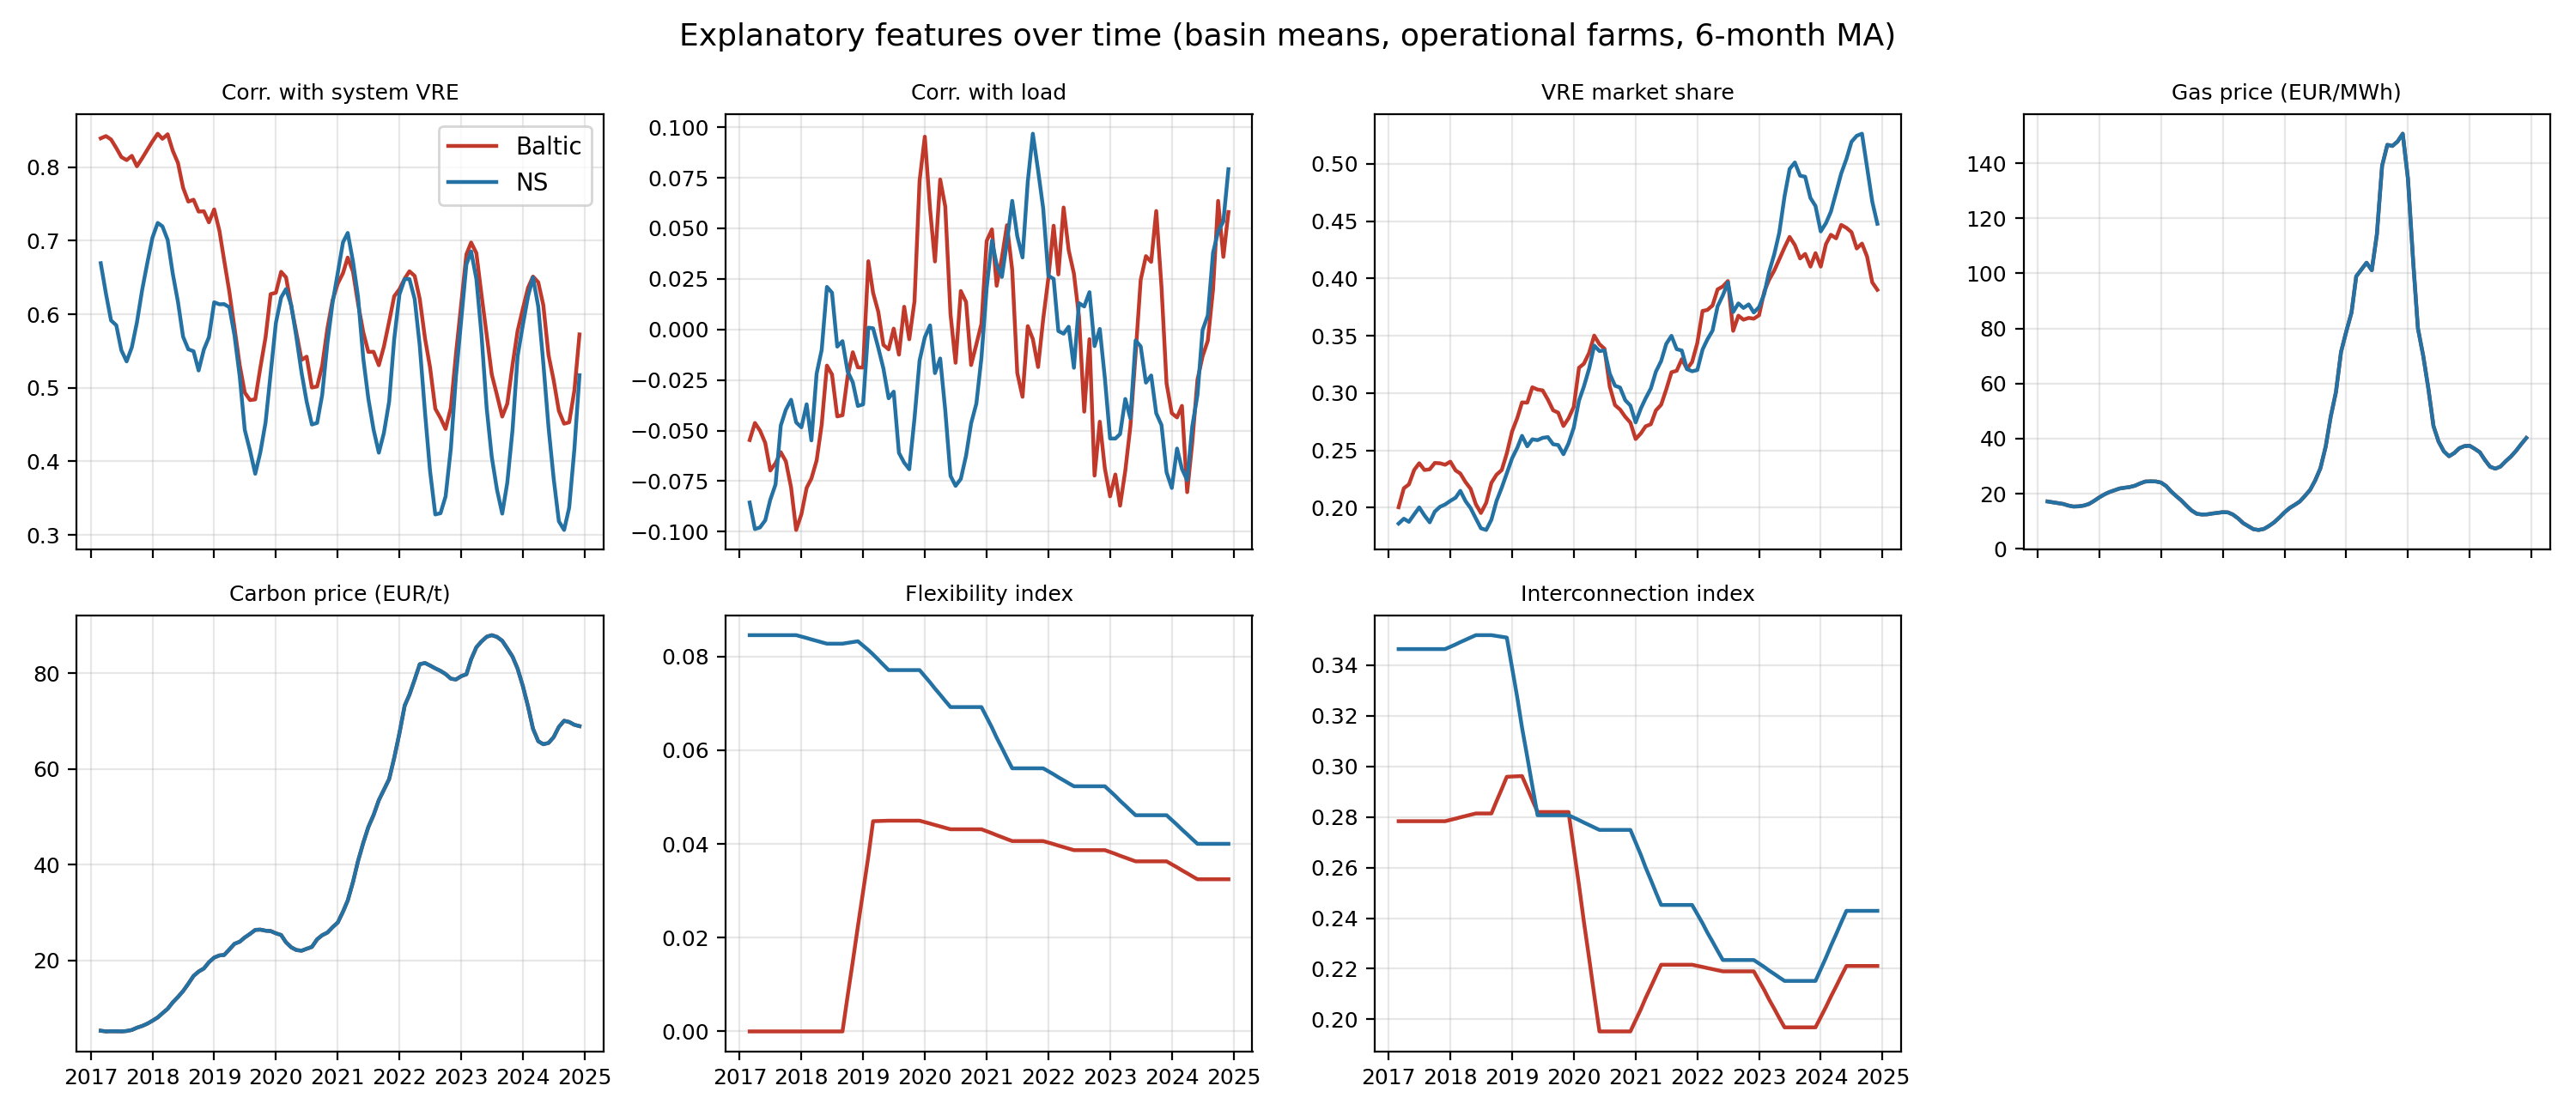
\includegraphics[width=0.98\textwidth]{fig_C_feature_evolution}
    \caption{Basin-mean evolution of the seven features for operational farms,
    2017 to 2024 (six-month moving averages). North Sea in blue, Baltic in red.}
    \label{fig:fig_C_feature_evolution}
\end{figure}

\subsubsection{Algorithm selection and validation}\label{sec:fitting}

In this work five algorithm families are tested: gradient boosting (XGBoost), random forests,
support vector regression, a degree-two polynomial, and ordinary least squares.
Their out-of-fold comparison is tabulated in Chapter~4
(Table~\ref{tab:algorithms}); gradient boosting is the strongest of the five
and carries the analysis.
The training unit is a bidding-zone market observation: a virtual farm at a
representative site in a zone, described by the seven features and labelled with
its monthly capture value. By the principle of Section~\ref{sec:currency} a zone
with observed prices is a valid observation whether or not a farm operates
there, so the panel is all 31 sites over 2017 to 2024, 2,706 zone-months. This
widens the enclosed Baltic from one operational price zone to seven. The
operational farms remain the validation subset. No hyperparameters are tuned, so
the comparison with Jacquet's untuned model is like for like.

How the primary model works also explains what it cannot do. Gradient boosting builds shallow decision trees in sequence, each fit
to the error the ensemble still makes and added at a small learning rate, so
nothing about the functional relationship is assumed in advance, and it
captures nonlinear interactions a single equation would miss, for instance that
interconnection lifts value only once penetration is high enough to need it. The cost of that flexibility is the limit described in
Section~\ref{sec:reg_projection}. A decision tree predicts by averaging the
training observations that fall in each of its leaves, so for an input beyond
the training range it can only return the value of its nearest boundary leaf,
giving a constant response. It interpolates well and does not extrapolate at
all, by construction, which is the reason a second model built from system
structure is needed for the future.

Validation is layered, because one scheme can flatter a panel model, and
all of them rest on one discipline, \textit{out-of-fold prediction}: a
prediction made by a model that never trained on that point. The schemes
differ only in what they withhold.

\begin{itemize}
    \item \textbf{Random five-fold cross-validation} withholds individual
    farm-months. It reproduces Jacquet's scheme, but for panel data it leaks:
    other months of the same farm stay in training, so the model is never asked
    about an unfamiliar farm.
    \item \textbf{Grouped five-fold cross-validation}, the headline scheme,
    withholds entire farms. Each farm-month is predicted by the one model copy
    blind to its farm, and the stitched series, every farm-month predicted once,
    is what all grouped metrics in Chapter 4 score.
    \item \textbf{A chronological split} trains through 2022 and tests on 2023 to
    2024. It withholds the future and stress-tests extrapolation across the
    post-crisis regime change.
    \item \textbf{Leave-one-year-out} fits on every other year and predicts the
    held-out one. Where the single chronological split conflates two failures,
    inability to forecast any year and inability to cross the 2021 to 2022 regime
    break, this separates them year by year, matching the multi-year temporal
    suites of both predecessors.
    \item \textbf{Basin-transfer fits} train on one sea and test on the other, to
    probe whether the learned relationships are basin-specific.
    \item \textbf{A variant excluding 2022} mirrors Jacquet's removal of the
    gas-crisis months.
\end{itemize}

The stitched out-of-fold series is exported for the three-way comparison: when
Section~\ref{sec:triangle} sets the regression against observation in a Danish
zone, the prediction comes from a model that never saw a Danish farm.

\subsubsection{Interpretation of the fitted model}\label{sec:mechanism_tools}

Two tools are used to read an explanation out of the fitted model. The first is
SHAP, short for SHapley Additive exPlanations, which splits each prediction into
a contribution from each of the seven quantities and is computed on the data the
model was fitted to.

SHAP gives the size of each contribution but not the shape of the relationship,
so Jacquet's analytical equation is refitted as the second tool
\cite{Jacquet2024}. Its starting point is that a farm selling in random hours
would have a capture value of one, and cannibalisation is what subtracts from
that one:
%
\begin{equation}
    \mathrm{CV} \;=\; 1
    \;-\; B\,\frac{M_{\mathrm{WF}}}{M_{\mathrm{BZN}}}\,S
    \;-\; C\,M_{\mathrm{WF}}\,
    \bigl(0.202\,p_{\mathrm{CO_2}} + p_{\mathrm{gas}}\bigr)^{\gamma},
    \label{eq:analytical}
\end{equation}
%
where $S$ is the renewable market share and $p_{\mathrm{gas}}$ and
$p_{\mathrm{CO_2}}$ are the monthly gas and carbon prices, folded together by
the emission intensity of gas. The first subtracted term represents cannibalisation through the pattern
penalty of Section~\ref{sec:features},
$M_{\mathrm{WF}} = \mathrm{sign}(\rho_{\mathrm{VRE}} -
\rho_{\mathrm{load}})\,|\rho_{\mathrm{VRE}} - \rho_{\mathrm{load}}|^{\alpha}$,
which grows when a farm's output follows the system's renewables more closely
than it follows demand, is scaled by the market share $S$, and is divided by
the buffering term
$M_{\mathrm{BZN}} = (I_{\mathrm{int}} + I_{\mathrm{flex}})^{\delta}$, in which
interconnection and flexibility absorb the surplus. The second subtracted term
represents the distortion of capture value by fuel prices.

Each constant controls one part of the mechanism: $\alpha$ sets how sharply the
penalty grows as a farm's output becomes more crowded, $B$ sets the overall
strength of the cannibalisation term, and $\delta$ sets how strongly
interconnection and flexibility protect against it. The constants are fitted
separately for each basin by least squares within fixed bounds, with confidence
intervals obtained by resampling whole farms; the fitted values are in
Appendix~\ref{app:assumptions}.

The fitted constants cannot be compared between the basins one at a time,
because different combinations of them produce almost the same curve: a
stronger crowding penalty, through a larger $\alpha$ or $B$, can be offset by
stronger buffering, through a larger $\delta$, and the fit cannot fully
separate the two. What the fit does pin down is the behaviour of the equation
as a whole. The two basins are therefore compared on what their fitted
equations predict, namely how much capture value falls when penetration rises,
calculated for both basins at the same market conditions so that the
comparison reflects the equations and never a difference in circumstances.

\subsubsection{Projection with the regression model: approach and limitations}
\label{sec:reg_projection}

Projecting a farm that has not been built means giving each of the seven
quantities a future value.

\begin{itemize}
    \item The two pattern correlations are held at the site's recent values,
    since they follow from its weather and its position on the grid
    \cite{Jacquet2024}.
    \item Penetration is scaled by the growth in renewable generation relative
    to the growth in demand in the TYNDP scenario.
    \item Gas and carbon prices are taken from the scenario.
    \item Flexibility grows with the battery fleet in the scenario.
    \item Interconnection is held at its recent value. This is mildly optimistic,
    since transfer capacity is unlikely to keep pace with wind, and a
    sensitivity is reported alongside.
\end{itemize}

Twelve sets of inputs are built for each year, one per month, and the predicted
capture values are averaged, so the projection keeps the site's own seasonal
pattern.

The decisive test is whether the model is being asked about conditions it has
seen. A projection is trusted only if all seven quantities lie inside the range
covered by the training data, because outside that range the model has nothing
to learn from.

A check on each quantity separately would be insufficient, however, because a
projection can sit inside the range of every quantity taken one at a time and
still be a combination that never occurred, as the seven do not vary
independently. A stricter test,
following Jacquet, asks whether the projection lies inside the region the
training data occupy in all seven dimensions at once, using its convex
hull. Where a projection fails, the prediction is repeated with the offending
quantity capped at its training maximum, which shows whether the answer depends
on the part of the range the model has never seen.

The equation of Section~\ref{sec:mechanism_tools} is exempt from this limit,
being a formula rather than a set of decision trees, and can therefore be
evaluated at any input, including values outside the
training range. It is projected on the same scenario inputs given to the system
model, which gives a third independent estimate. It differs from Jacquet's use
of it in one way. He holds the pattern correlations fixed, whereas in this work the
Baltic projection lets the correlation with system wind rise towards the level
the built-out Baltic zones already show, and lets interconnection utilisation
fall as wind grows faster than transfer capacity
(Appendix~\ref{app:assumptions}).

\subsection{The system model (PyPSA-Eur)}\label{sec:system}

\subsubsection{Price formation in PyPSA-Eur}\label{sec:pypsa_how}

PyPSA-Eur is the European configuration of PyPSA \cite{Horsch2018}, an open
workflow that assembles a model of the European power system from public data.
The transmission grid comes from ENTSO-E maps, the power plants from open
databases, the weather from the same ERA5 data used for the virtual wind farm,
and demand from historical load. The thousands of connection points in the real
grid are grouped into a smaller number of representative nodes, which is the
setting that trades spatial detail against the size of the problem to be solved.

The model finds the cheapest way to meet demand in every hour of a year, subject
to the capacity of every plant and every line. That problem is a linear program,
so the solution found is the true optimum rather than a good approximation, even
with tens of millions of variables. It is solved with the barrier algorithm in
Gurobi.

Two of its outputs are used in this thesis. The first is how much every generator produces
in every hour. The second is the shadow price at every node, which is what it
would cost to serve one more unit of demand there in that hour. In a windy hour
the last unit needed comes from wind, which costs almost nothing to run, so the
price falls towards zero. In a still hour it comes from a gas plant, which sets
a much higher price. A real market clearing on marginal cost prices in the same
way, which is why the shadow price is used as the wholesale price.
Practical details are in Appendix~\ref{app:assumptions}.

\subsubsection{Scope and configuration}\label{sec:pypsa_config}

The model covers the fourteen countries around the two basins. They are
clustered into thirty nodes, with more nodes given to the markets that carry
most of the offshore wind, and solved at full hourly resolution. Thirty nodes is
finer than one node per country, so Denmark separates into its two  bidding
zones, and congestion within a zone as well as between zones is priced at each
node.\footnote{In a zone represented by more than one node, the denominator of
capture value is the price averaged across that zone's nodes, which corresponds
to the single zonal price of Equation~\ref{eq:value_factor}, while the numerator
weights each generator by the price at its own node. The two are identical
wherever offshore wind is present at all of a zone's nodes, which is the case in
the single-node Baltic zones that carry the headline result. A difference arises
only in zones that also contain inland nodes with no offshore wind.}

Transmission is held at today's capacity throughout. Congestion is
priced as it exists now, which
makes the projection conservative. Section~\ref{sec:robustness} solves the
opposite case, with transmission free to expand.

Generation fleets are set to the capacity installed in each modelled
year, and topped up where the database falls short of national statistics. For
2023 and 2024, fuel and carbon prices are set to the observed annual
averages.

\subsubsection{Historical baselines and calibration}
\label{sec:calibration_method}

Three past years are solved. 2023 is the main validation year. 2019 is added so
that the model is tested both before and after the energy crisis, in a cheap-gas
world and an expensive one. 2024 is added because it provides validation points
at the highest penetrations yet observed, which is what the bias correction of
Section~\ref{sec:bias_method} is fitted on.

The calibration is judged on price levels and on capture value. Price levels
are compared zone by zone against observed
day-ahead prices, using a normalised absolute error, because percentage errors
are undefined when prices are negative. Capture value, the quantity the thesis
uses, is checked separately, and a third value is calculated alongside it to
locate any error: the model's own generation valued at observed prices. If that
hybrid value matches observation while the fully modelled value does not, the
modelled prices carry the error and the modelled generation is sound.

Solver settings are the same for the past years and for the projections, so the
bias correction is applied to prices formed in exactly the same way as the ones
it was fitted on. The settings are listed in Appendix~\ref{app:assumptions}.

\subsubsection{Projection to 2030 and 2040}\label{sec:projection}

The projection solves six scenarios from the 2024 TYNDP trajectories on the
validated 2023 network. Four follow National Trends, the pathway that tracks
existing national policies: for each of 2030 and 2040, one solve installs the
Baltic offshore capacity the plan schedules, and one an accelerated variant in
which the Baltic builds further. The remaining two repeat the accelerated 2040
case under the plan's other demand pathways, Distributed Energy and Global
Ambition, which electrify more of Europe's energy demand. All six are listed
with their results in Table~\ref{tab:projection}.

Two assumptions govern demand. The base year is 2019, the last year before the
crisis depressed consumption, and demand in each scenario year is that base
scaled by the country's TYNDP growth factor, with documented substitutes for
the two countries the scenario tables omit. Capacity targets are adopted in
full: where a scenario prescribes more capacity than the clustered nodes can
physically host, the whole target is still installed and the excess is
recorded, so no capacity is dropped without record.

Six further corrections close the remaining gaps between renewable-only
scenario tables and an electricity-only model, and Table~\ref{tab:corrections}
states each with its implementation and rationale. All act in the same
direction, preventing the model from generating surplus zero-cost electricity
that would make capture value look higher than it should be.
\begin{table}[H]
\centering
\small
\caption{The six corrections, labelled A to F, applied to the scenario inputs
before the 2030 and 2040 solves. The TYNDP scenario tables prescribe renewable
capacity only and the system model represents the electricity sector only, so
each correction closes a gap that combination leaves open. Each row states
what is changed and why.}
\label{tab:corrections}
\begin{tabular}{l >{\raggedright\arraybackslash}p{10.8cm}}
\toprule
\textbf{Correction} & \textbf{What is changed, and why} \\
\midrule
A. Coal phase-out & German and Polish coal and lignite capacity is reduced
year by year in line with the legislated closure schedules, which the scenario
tables leave out. \\
\addlinespace
A2. Polish nuclear & Poland's announced 3.9~GW nuclear programme is added from
2040, since the scenario tables add no thermal capacity at all. \\
\addlinespace
B. Offshore caps & Danish, Finnish and Swedish offshore capacity is capped at
the nationally planned levels, removing capacity that the scenario tables
wrongly assign to these zones through planned energy islands. \\
\addlinespace
C. DK1/DK2 split & The Danish offshore total is split 60/40 between the DK1
and DK2 bidding zones by 2040, because the default allocation by wind resource
alone gives DK2 too little. \\
\addlinespace
D. Hydrogen demand & Electrolysers with a fixed hydrogen demand are added in
each country, alongside a priced import alternative that sets the level at
which producing hydrogen is worthwhile. This gives surplus electricity a use;
without one, an electricity-only model produces implausibly many hours priced
at zero. \\
\addlinespace
E. Demand base year & Demand is projected from a 2019 base using the TYNDP
growth factors, with documented substitutes where factors are missing, because
the factors are quoted relative to 2019 and two countries are absent from the
scenario tables. \\
\addlinespace
F. Shortage pricing & Demand response is added at 5\,\% of peak load, offered
at 400~\euro/MWh, with involuntary curtailment at the 4{,}000~\euro/MWh price
cap, so that hours of shortage are priced the way a real auction prices them. \\
\bottomrule
\end{tabular}
\end{table}
\subsection{Validation against observed prices}\label{sec:confrontation}

\subsubsection{Comparison with observed ENTSO-E prices}\label{sec:triangle}

For every zone and year in which offshore generation was observed,
which is five zones across 2019, 2023 and 2024, the same capture value is
estimated three times: from observation, by the system model, and by the
regression model. The regression estimate comes from a copy that never saw that
zone's farms.

These three estimates are mutually independent, since the regression estimate
uses nothing from the farm it is predicting, the system estimate uses no
market prices at all, and the observed value comes from outside both models.
Agreement between them is therefore informative, and where they disagree, the pattern of the
disagreement shows which model is at fault. This is a different exercise from
the hybrid value of Section~\ref{sec:calibration_method}, which
mixes modelled generation with observed prices in order to locate an error
inside the system model.

\subsubsection{Bias correction procedure}\label{sec:bias_method}

The comparison above shows the system model reading high in small congested
zones, and by more where more offshore wind has been built (Chapter 4). That
relationship is what the correction uses. A straight line is fitted by least
squares through the measured overstatements against the zone's offshore
penetration, meaning its offshore generation as a share of consumption, and the
fitted line is subtracted from the model's output:
%
\begin{equation}
    \mathrm{CV}_{\mathrm{corr}} = \mathrm{CV}_{\mathrm{raw}}
    - \bigl(\hat{a} + \hat{b}\,\pi\bigr),
    \label{eq:bias}
\end{equation}
%
where $\pi$ is the zone's modelled offshore penetration and $\hat{a}$ and
$\hat{b}$ are the fitted intercept and slope. The model's own penetration is
used, not the observed one, because the correction is applied to the model's
own output. This quantity is narrower than the all-renewables share used as a
feature by the regression model.

\subsubsection{Decomposition and scoring of the difference between the models}
\label{sec:gap_method}

Section~\ref{sec:triangle} establishes that the two models differ and four further
tests establish why: where they agree, where they part, how each compared
to the observed counterparts, and how their projections compare.

\textbf{Channel decomposition.} Both models compute capture value with the same
formula (Equation~\ref{eq:value_factor}) from different inputs. The regression
model uses the virtual farm's generation valued at observed day-ahead prices,
and the system model uses its own generation valued at its own prices.
Substituting one input at a time, and averaging over both possible orders,
divides the difference between their answers exactly into a generation part and
a price part, with nothing left over and no dependence on which substitution is
made first. The price part divides again by re-pricing against observed prices
with negative values set to zero, which isolates the effect of the linear
program being unable to produce them. A fourth part carries the way the network
is represented, and a small remainder absorbs the out-of-fold fit and the
averaging of prices across nodes.

\textbf{Scoring both models on targets neither has seen.} Comparing the two
directly would favour the regression model, since it is fitted to the record it
would be scored on. It is therefore refitted with the target withheld, using the
grouped schemes of Section~\ref{sec:fitting}, once leaving out each bidding zone
and once leaving out each year. Whole blocks are withheld rather than individual
observations, because capture value is correlated in space and in time, and
withholding single points would leave near-duplicates in the training set
\cite{Roberts2017}. Both models are then scored on the same zone-months against three measures.

Mean absolute error and root mean squared error are
reported on the natural scale of capture value, which is dimensionless and
bounded, so the usual objections to percentage errors do not apply
\cite{HyndmanKoehler2006}. Signed bias records the direction of each model's
error. A skill score compares both against the benchmark of assuming that a farm
simply earns the average price. Because zone-months within a zone are not
independent, the difference between the two models is tested by a paired
comparison with a bootstrap that resamples whole zones \cite{DieboldMariano1995}.

Accuracy alone would not settle the question, since two models can be equally
accurate and have different errors. Each model's error is also separated,
following Theil \cite{Theil1966}, into three parts: a consistent offset, a
failure to match how much the observations vary, and mistiming, which is the
error that remains once level and spread are both right. The arithmetic is in
Appendix~\ref{app:forecast_checks}.

\textbf{Backtesting the projection.} The test above scores the models but not
the act of projecting, which also requires future inputs to be built. The
regression model is therefore refitted on data up to 2021 and asked for 2023 and
2024 twice: once from the inputs that occurred, and once from inputs
constructed the way a projection must construct them, with weather terms set to
each farm's pre-2022 average and system terms carrying the pre-2022 monthly
shape. The system model is fitted to nothing, so it is already a projection, and
it is scored on the same targets. The difference between the two regression runs
is the cost of building the inputs, and the difference between either of them
and the system model is the like-for-like comparison. The constructed inputs use
the annual levels that occurred, and not those a forecaster in 2021 would have
assumed, so the test grants perfect foresight of the scenario.

\textbf{Comparing the two projections.} Both models are run on the same TYNDP
scenarios, so the only difference between their answers is the model. They are
compared at 2030, where both are still inside the observed range, and at 2040,
where the regression model is not. Because 2040 cannot be checked against
observation, both projections are also placed beside published estimates of
capture value at high penetration, recording the renewable share at which each
published figure was measured. Recording that share matters, because a benchmark measured at a share on which
the regression model was trained cannot separate the two models, since a model
reproducing conditions inside its training range will match it regardless of
its behaviour beyond that range, and only a benchmark from an already
saturated market is decisive.

\textbf{The exclusion of DK2.} DK2 is left out of the scored set, on a criterion
fixed before the results were seen. Its prices are set partly by plants that
must keep running and by combined heat and power, neither of which a linear
program represents, and this shows in its 264 observed hours of negative prices
in 2023 against the system model's zero. It remains in the regression model's
training data, and every headline figure is also reported with DK2 included.

\subsubsection{Robustness, model runs and reproducibility}\label{sec:robustness}

The projected values rest on assumptions about fuel prices, the transmission
grid, the pricing of shortage, and the six scenarios chosen, and the
sensitivity of the results to each of these is tested in turn.

\begin{itemize}
    \item \textbf{Gas prices.} The assumed gas price is varied by re-solving
    three buildouts across five gas prices, which separates the effect of the
    buildout from the effect of fuel costs.
    \item \textbf{Transmission.} The grid assumption is inverted by re-solving
    all six scenarios with transmission free to expand, which gives the bound
    opposite to the grid held at today's capacity
    (Section~\ref{sec:pypsa_config}).
    \item \textbf{Shortage pricing.} The treatment of shortage is tested by
    recalculating every capture value with the shortage-priced hours removed,
    meaning those in which supply is tight and the price rises to the levels
    set by demand response or the price cap, which establishes that the result
    does not rest on a few extreme prices.
    \item \textbf{Scenario choice.} The dependence on the six chosen scenarios
    is tested with a fast approximation of the system model, trained on 76
    solved networks, which prices a scenario in milliseconds and so allows far
    more scenarios to be examined than could be solved directly.
\end{itemize}

The results of all four sensitivity analyses, together with the validation of
the fast approximation, are collected in Appendix~\ref{app:robustness}.

Every model run behind Chapter 4 is listed in Table~\ref{tab:runs} of
Appendix~\ref{app:repro}, so each number can be traced to the run that produced
it, and the whole procedure is scripted from the raw downloads to the final
tables. A single command re-solves everything in about three hours, every
reported number can be regenerated from public data, and the solver settings
and assumptions are fixed in Appendix~\ref{app:assumptions}.



\subsection{Value-adjusted cost of energy}
\label{sec:vlcoe_method}

Capture value on its own does not tell an investor whether to build, so this
section turns it into a cost. The measure used is the value-adjusted levelised
cost introduced in Section~\ref{sec:vlcoe_lit}: the levelised cost divided by
capture value, which gives the average wholesale price a site must earn to break
even. It is used because capture value enters it directly, so a projected
fall in value becomes a rise in the price a site needs.

\subsubsection{Mapping levelised cost}\label{sec:cost_field}

Costs are mapped at the resolution of the wind resource rather than that of the
system model. Three geospatial datasets are used: capacity factor from the
Global Wind Atlas at roughly two kilometres \cite{GlobalWindAtlas}, water depth
from GEBCO \cite{GEBCO2014}, and distance to shore, calculated on the same grid.

Capital cost rises with both depth and distance, since deeper water requires heavier
foundations, with a step change beyond 60 metres where fixed-bottom foundations
give way to floating ones, and sites further from shore require longer export
cables. Capital cost is modelled in segments, one for each of these
regimes, anchored to the PyPSA-Eur cost database and IRENA's 2024 review
\cite{Horsch2018, IRENA2025Costs} and set out in
Appendix~\ref{app:assumptions}. It is annualised at a 7\,\% cost of capital over
a life of 27 to 30 years.

The levelised cost is the annualised cost divided by the energy a megawatt of
capacity delivers in a year,
%
\begin{equation}
  \mathrm{LCOE}(d,\ell,y) \;=\;
  \frac{\mathrm{CRF}\,\lambda(y)\,\mathrm{CAPEX}(d,\ell) + f_{\mathrm{OM}}(\ell)}
       {\mathrm{CF}\cdot 8760},
  \label{eq:lcoe}
\end{equation}
%
and it is computed for every cell at all three years. The full set of maps is in
Appendix~\ref{app:atlas}.

\subsubsection{Combining cost with capture value}\label{sec:vlcoe_def}

The value-adjusted cost (Equation~\ref{eq:vlcoe}) is calculated for each cell by
dividing its levelised cost by the capture value of the zone it sits in, taken
from the solved networks.

The same inputs give a second quantity, the net value of a site, which is the
revenue it captures less its annualised cost,
%
\begin{equation}
  \mathrm{NV}(d,\ell,y) \;=\;
  \underbrace{\mathrm{CF}\cdot 8760\cdot \mathrm{CV}\cdot \bar p}_{\text{captured revenue}}
  \;-\; \big(\mathrm{CRF}\,\lambda(y)\,\mathrm{CAPEX} + f_{\mathrm{OM}}\big).
  \label{eq:netvalue}
\end{equation}
%
The value-adjusted cost says what price a site needs. The net value says how
much money it makes or loses at a given price. Both are reported for a merchant
project, meaning one that sells at market prices with no support contract.

\subsubsection{Pricing interconnection and robustness checks}\label{sec:vlcoe_grid_method}

Capture value enters the denominator of the value-adjusted cost, so any change
in capture value changes the average wholesale price at which a site's
revenues cover its costs. The effect of transmission on that break-even price
is isolated by computing Equation~\ref{eq:vlcoe} for 2040 twice, once with the
per-zone capture values of the grid held at today's capacity and once with
those of the grid free to expand, while the levelised cost is held identical
in both. Transmission is a separate investment that leaves the cost of
building and operating a farm unchanged, so only the revenue side of the
calculation moves, through capture value, and the difference between the two
computations is reported for each basin as the reduction in the break-even
price, in \euro/MWh.

Whether the value-adjusted cost rises or falls to 2040 is then tested across 27
combinations of three cost assumptions: the weighted average cost of capital at
5, 7 and 9\,\%, a multiplier on capital cost of 0.8, 1.0 and 1.2, and a 2040
learning rate of 5, 12 and 25\,\%. The absolute cost level cancels when the 2040
value-adjusted cost is divided by the 2025 one, so the direction depends only on
whether cost falls faster than capture value. That same ratio also gives
directly the rate of cost decline that would be needed to hold the
value-adjusted cost flat.

\subsection{Methodological justification}\label{sec:method_why}

Each choice above follows from one of the research questions.

\begin{itemize}
          \item \textbf{Two models rather than one}, to compare them and decide
    which is better suited to representing the present and forecasting the
    short term, and which to forecasting the long term.
    \item \textbf{Gradient boosting for the regression model}, because it scores
    best of the five algorithms tested (Table~\ref{tab:algorithms}), and because
    the way it fails is visible: beyond its training range it returns a
    constant, which can be detected and reported.
    \item \textbf{PyPSA-Eur for the system model}, because it is the only option
    combining open code and open data, the full European network, resolution at
    the level of bidding zones, and hourly dispatch.
    \item \textbf{Every scenario solved twice}, with the grid at today's
    capacity and with it free to expand, because the difference between the two
    isolates the part of the erosion caused by congestion, which is what the
    second research question asks.
    \item \textbf{The value-adjusted cost}, because it carries the measured
    capture value into the decision an investor makes.
\end{itemize}

The limits of each of these choices are recorded in
Appendix~\ref{app:assumptions}.